\documentclass[french]{beamer}
% \setbeamertemplate{navigation symbols}{}

\usepackage[utf8]{inputenc}
\usepackage[T1]{fontenc}
\usepackage{graphicx}
\usepackage{tabularx}

\usepackage{xcolor}

\usetheme{Hannover}
\useoutertheme{infolines}
%%%%%%%%
\makeatletter
\beamer@nav@subsectionstyle{show/show/hide}
\makeatother


% \usepackage{siunitx}
% \usepackage[]{algorithm2e}

\usepackage{caption}
\captionsetup{font=scriptsize,labelfont=scriptsize}
\setbeamertemplate{caption}[numbered]

\usepackage{amsmath}
\DeclareMathOperator{\sinc}{sinc}
\DeclareMathOperator{\e}{e}
\setbeamerfont{caption}{size=\footnotesize}


\title[Soutenance MT3]{Etude de la nutation de la terre par analyse de données VLBI}
\author[Hottier.C, Nurulhuda.I, Robert.C]{Hottier.C, Nurulhuda.I, Robert.C\\dirigés par Lambert.S}
\date{4 mars 2016}


\newcommand{\frtt}[1]{\frametitle{#1}}
\newcommand{\FIXME}[1]{\textcolor{red}{FIXME : #1}}

\graphicspath{{Figures/}}

\begin{document}


\begin{frame}
  %\titlepage % Print the title page as the first slide
  \maketitle
  \begin{center}
    
\includegraphics[height=0.20\textheight]{Figures/siteon0.jpg}
    %\hspace{8.5cm}
  \end{center}
\end{frame}

\begin{frame}
  \frametitle{Sommaire}
  \tableofcontents
\end{frame}


\section{Introduction}

\begin{frame}
  \frtt{Introduction}

  \begin{itemize}
    \item \'Etude de la nutation de la terre 
    \item Modèle de terre :
      \begin{itemize}
        \item Surface déformable
        \item Manteaux rigide
        \item Noyaux fluide
      \end{itemize}
  \end{itemize}

\end{frame}




\section{Mouvement du pôle et fonction de transfert}

\begin{frame}
  \frtt{Lien entre Terre rigide et modèle avancé (MHB)}
   REN (\textit{Rigid Earth Nutation}) et nutation observée reliées par une fonction de transfert :
   \begin{align*}
     \frac{\tilde{\eta}_{MHB}}{\tilde{\eta}_{REN}}(\sigma) 
     \equiv \tilde{T}(\sigma) 
     = \frac{e_R\Omega-\sigma}{e_R\Omega} &\left[ \kappa - \frac{A_f}{A}\gamma\right.- \frac{\Omega(e-\kappa)}{\sigma-\frac{A}{A_m}\Omega(e-\kappa)}\\
     &-\left. \frac{A_f}{A_m} \frac{\Omega (e-\gamma)(e_f-\beta)}{\sigma + \Omega(1+ \frac{A}{A_m}(e_f-\beta))}\right]
   \end{align*}
   	\onslide<2> \textbf{Objectif de la méthodo :} 
   	\\ajustement de cette fonction sur les paramètres géométriques (excentricité, déformation...) du noyau. 
\end{frame}


\begin{frame}
  \frtt{}
\end{frame}




\section{Données observationnelles}

\begin{frame}
  \frtt{Observation VLBI}
\end{frame}




\section{Analyse des données}

\begin{frame}
  \frtt{Analyse des données}
Données: \\
	\begin{itemize}
		\item VLBI Earth Orientation Solution OPA2015a	
		\item Rigid Earth Nutation (Souchay et al. 1997)
	\end{itemize}
	\vspace{0.5cm}
	L'équation des moindres carrés: \\
	$X(t) + i \times Y(t) = \sum\limits_{j=1}^{40} (\widetilde{A}_{j} \times e^{(\omega_{j}*t + \varphi_{j})})$ \\
	$\widetilde{A} = A_{Re} + i \times A_{Im}$ \\

	\vspace{0.5cm}
	$\widetilde{A}$ : amplitude \\
	$\omega$ : fréquence \\
	$\varphi$ : phase \\
	$t$ : temps
\end{frame}

\begin{frame}
  \frtt{Amplitude Ajustées}
	\begin{center}
		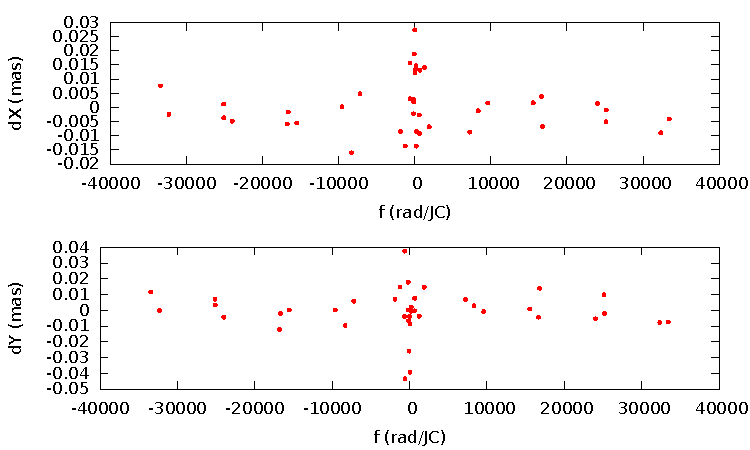
\includegraphics[width=1.0\textwidth]{amplitude_freq.pdf}
	\end{center}
\end{frame}

\begin{frame}
  \frtt{Comparaison entre série ajusté et observation}
	\begin{center}
		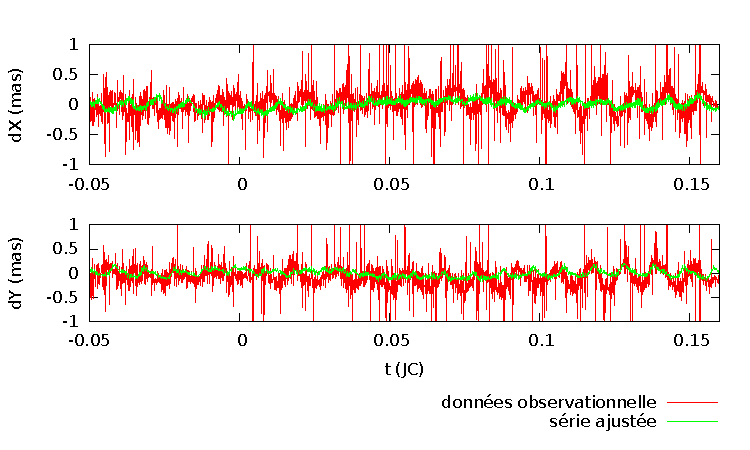
\includegraphics[width=1.0\textwidth]{fit_amplitude_ser_obs.pdf}
	\end{center} 
\end{frame}



\section{Mouvement Libre}
\begin{frame}
  \frtt{Mouvement Libre}
\end{frame}



\section{Résultats}

\begin{frame}
	\frtt{Ajustement de $\tilde{T}$}
	
	\begin{figure}
	\centering
	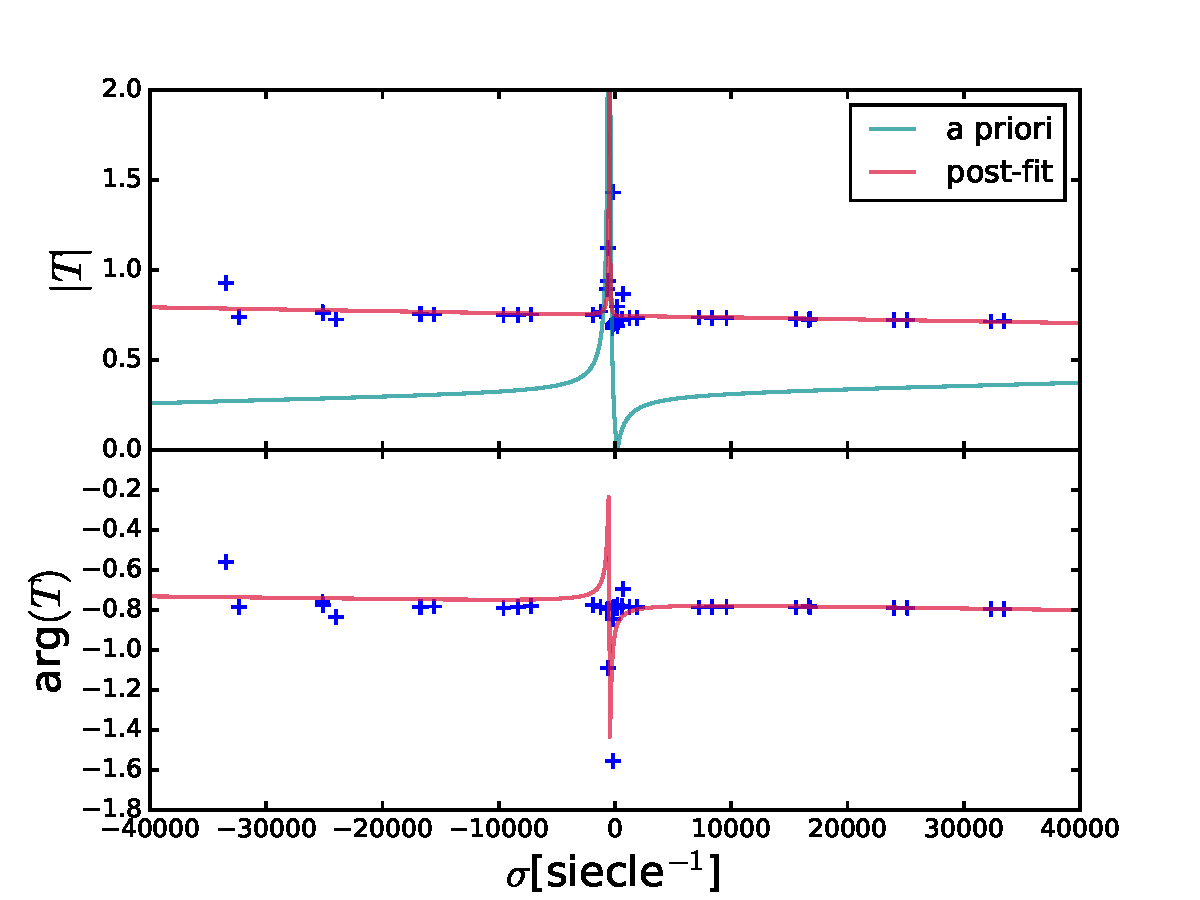
\includegraphics[width=0.9\textwidth]{fit_transfert.pdf}
	\end{figure}

\end{frame}

\begin{frame}
\frtt{Importance des corrections}
\begin{figure}
\begin{tabular}{cccc}
param & a priori & correction post-fit & |correction relat|\\
\hline
$\kappa$ & $1.039e-2$ & $(-1.3+1.6i)e-2$ & $20.3$ \\
%\hline
$\gamma$ & $1.965e-2$ & $(-1.4+1.5i)e-2$ & $10.2$ \\
%\hline
$e$ & $3.257e-2$ &$-0.015+1.5i$  & $6.4$ \\
%\hline
$(e_f-\beta)$ & $1.931e-2$ & $(-0.58-1.1i)e-4$ & $6.5e-2$ 
\end{tabular}
\end{figure}
\centering
   
    

\end{frame}

\section{Conclusion}

\begin{frame}
  \frtt{Conclusion}
\end{frame}


\end{document}
